\documentclass[UTF8]{ctexart}
\usepackage{graphicx}
\usepackage{amsmath}
\usepackage{amssymb}
\usepackage{graphicx}
\usepackage{geometry}
\geometry{left=3.0cm,right=3.0cm,top=3.5cm,bottom=2.5cm}
\everymath{\displaystyle}
\usepackage{float}
\usepackage{setspace}
\setstretch{1.25} 
\usepackage{float}
\usepackage{bookmark}
\begin{document}

\section{Probability and Stochastic Process}

\subsection{Probability}

$\operatorname{Var}X = \mathbb{E}[(X-\mathbb{E}X)^2] = \mathbb{E}[X^2]-(\mathbb{E}X)^2$.
$\operatorname{Var}(aX+b) = a^2 \operatorname{Var}X$.

$\operatorname{Cov}(X,Y) = \mathbb{E}[(X-\mathbb{E}X)(Y-\mathbb{E}Y)] 
= \mathbb{E}[XY]-\mathbb{E}[X]\mathbb{E}[Y]$.
$\operatorname{Cov}(aX+b,Y) = a\operatorname{Cov}(X,Y)$.

Cov Matrix for $X=(X_1,\dots,X_n)^T$: $\operatorname{Cov}(X) = (\operatorname{Cov}(X_i,X_j))_{i,j}$.

$\operatorname{Corr}(X,Y)=\frac{\operatorname{Cov}(X,Y)}{\sqrt{\operatorname{Var}X \operatorname{Var}Y}}$

矩母函数 Moment generating function: For rv $X$, MGF is $M_X(t)=\mathbb{E}[e^{tX}]$.
For vec-valued rv $\mathbf{X}$, $M_X(\mathbf{t})=\mathbb{E}[e^{\langle \mathbf{t},\mathbf{X} \rangle }]$.
可以生成$n$阶矩 $\mathbb{E}[X^n]=\frac{d^n}{dt^n}M_X \Big| _{t=0}$. 矩母函数相同说明分布相同.


特征函数 Ch.f.: For rv $X$, $\varphi_X(t)=\mathbb{E} [\exp(itX)]$.
For vec-valued rv $\mathbf{X}$, $\varphi_X(\mathbf{t})=\mathbb{E}[e^{i \langle \mathbf{t},\mathbf{X} \rangle }]$.

\noindent \textbf{一些分布}
\begin{itemize}

\item Binomial$(p, n)$: $P_X(k)=C_n^k p^k (1-p)^{n-k}$. 期望$np$, Var $np(1-p)$.
\item Poisson$(\lambda)$: $P_X(k)=e^{-\lambda}\frac{\lambda^k}{k!}$. 期望$\lambda$, Var $\lambda$.
\item Normal$(\mu, \sigma^2)$: $f_X(x)=\frac{1}{\sqrt{2\pi\sigma^2}}\exp(-\frac{(x-\mu)^2}{2\sigma^2})$. 偏度为0, 峰度为3. MGF: $\exp (\frac12 u^2 t)$.
\item Exponential$(\lambda)$: $f_X(x) = \lambda e^{-\lambda x}(x\geq 0)$. 期望$\lambda$, Var $\lambda^2$.

\end{itemize}

\noindent \textbf{Multivariate Gaussian} $\mathcal{N}(\mu,\Sigma)$

定义: Random vec $X$是$d$维Gaussian Vec 若对任意$t\in\mathbb{R}^d$, $\langle t,X \rangle $都是Gaussian.

Note that $n$个正态分布拼起来不一定是Gaussian vec, 但$n$个独立正态分布拼起来一定是.

给定vec $\mu$和半正定对称阵$\Sigma$, 存在Gaussian Vector $X$ with mean $\mu$ and Cov $\Sigma$.
如果$\Sigma$是满秩的, 则存在density
$f(\mathbf{x}) = (2 \pi)^{-d / 2} \operatorname{det}(\boldsymbol{\Sigma})^{-1 / 2} \exp \left(-\frac{1}{2}(\mathbf{x}-\boldsymbol{\mu})^{\mathrm{T}} \boldsymbol{\Sigma}^{-1}(\mathbf{x}-\boldsymbol{\mu})\right)$,

MGF  $\exp \left( \mu^T t + \frac{1}{2} t^T \Sigma t \right)$.
ChF $\exp \left( i \mu^T t - \frac{1}{2} t^T \Sigma t \right)$.

条件概率: $\mathbb{P}(A|B)=\frac{\mathbb{P}(A\cap B)}{\mathbb{P}(B)}$.
贝叶斯公式: $\mathbb{P}(A|B) = \mathbb{P}(B|A) \frac{\mathbb{P}(A)}{\mathbb{P}(B)}$.

条件期望: 
$\mathbb{E}[X|\mathcal{F}]$是一个随机变量使得
(1)是$\mathcal{F}$可测的; 
(2)$\mathbb{E}[\mathbb{E}[X|\mathcal{F}]1_A]=\mathbb{E}[X 1_A], \forall A \in\mathcal{F}$.

对两个rv $X,Y$, 有joint density $f_{X,Y}(x,y)$, 则Marginal density $f_X(x)=\int_{\mathbb{R}} f_{X,Y}(x,v)dv$.
条件密度 $f_{X|Y}(x|y) = \frac{f_{X,Y}(x,y)}{f_Y(y)}$,
条件期望 $\mathbb{E}[X|y]=\int_{\mathbb{R}}xf_{X|Y}(x|y)dx$.
$\mathbb{E}[g(X)|Y]=h(Y)$ where 
$h(y) = \frac{\int g(x)f_{X,Y}(x,y)dx}{\int f_{X,Y}(x,y)dx}$.

独立性引理. 若$X, Y$独立, 则$\mathbb{E}[\varphi(X,Y)|Y]=h(Y)$ where
$h(y)=\mathbb{E}[\varphi(X,y)]$.
更一般地, $X_1,\dots,X_k$是$\mathcal{G}$可测的, $Y_1,\dots,Y_l$独立于$\mathcal{G}$,
则$\mathbb{E}[f(X_1,\dots,X_k,Y_1,\dots,Y_l)|\mathcal{G}]=g(x_1,\dots,x_k)$
where $g(x_1,\dots,x_k)=\mathbb{E}[f(x_1,\dots,x_k,Y_1,\dots,Y_l)]$.

\noindent \textbf{一些命题}
\begin{itemize}

\item $F$递增+右连续+$[0,1]$,即可定义一个分布函数. 
如果存在非负$f$使$F(t)=\int_{-\infty}^t f(x)dx$, 则分布有density.

\item $X$有pdf $f_X$, $Y=g(X)$其中$g$可微且严格单调, 则$f_Y(y)=f_X(g^{-1}(y))\frac{d}{dy}g^{-1}(y)$.

\item $X\sim \mathcal{N}(\mu,\sigma^2)$,
则$\mathbb{E}[|X|]=\mu\left[2 \Phi\left(\frac{\mu}{\sigma}\right)-1\right]+
\frac{2 \sigma}{\sqrt{2 \pi}} \exp \left\{-\frac{\mu^{2}}{2 \sigma^{2}}\right\}$.
其中$\Phi$为std norm CDF.

\item 在$[0,1]$的均匀分布下取$n$个值, 最大值的期望是$\frac{n}{n+1}$.

\item Distribution of $X+Y$ when $X\sim f,Y\sim g$ are independent:
$\mathbb{P} (X+Y\leq z)=\int\mathbb{P}(x\leq z-y)g(y)f(y)dy$,
density of $X+Y$ is $h(z)=\int f(z-y)g(y)dy$.

\item 顺序统计量 $k$th order statistic: the $k$th smallest value in a sample of $n$ from a random distribution.
There is $\mathbb{P}(X_{(k)}\leq x)=\sum_{j=k}^n F(x)^j (1-F(x))^{n-j}$.

\end{itemize}

大数定律: 
$X_1,\dots,X_n$ 是 iid rv 序列, 期望$\mu$有限.
令 $S_n = X_1+\dots+X_n$, 则 
(弱) $\frac{S_n}{n}\to\mu$ in probability i.e.
$\lim_{n\to\infty}\mathbb{P}(|\frac{S_n}{n}-\mu|>\varepsilon)=0$.
(强) Almost surely $\lim_{n\to\infty}\frac{S_n}{n}=\mu$.

中心极限定理 Central Limit Theorem: 
$X_1,\dots,X_n$ 是 iid rv 序列, 期望$\mu$和方差$\sigma^2$有限,
令 $S_n = X_1+\dots+X_n$, 则 $Y_n=\frac{S_n-\mu n}{\sigma\sqrt{n}}$
converges in distribution to std norm.


\subsection{Stochastic Process}

\noindent \textbf{鞅和停时}

$(X_n)$ or $(X_t)$是鞅, $T$是停时, 则$(X_{n\wedge T})$ or $(X_{t\wedge T})$是鞅.

[Optional Stopping Thm] $(X_n)$ u.i. sub-mtg, $S\leq T$是停时, 则$\mathbb{E}[X_T|\mathcal{F}_S]\geq X_S$.
$(X_t)$ u.i. mtg, $S\leq T$是停时, 则$\mathbb{E}[X(T)|\mathcal{F}(S)]=X(S)$.

Rk. 一致可积u.i.即$\forall \varepsilon, \exists K$ s.t. $\mathbb{E}[|X_n|1_{|X_n|\geq K}]<\varepsilon (\forall n)$.
对离散sub-mtg, 一致可积$\Leftrightarrow$ convergence a.s. and in $L^1$  $\Leftrightarrow$ convergence in $L^1$.
对连续mtg, 一致可积$\Leftrightarrow$ convergence in $L^1$  $\Leftrightarrow$ $\exists Y\in L^1, X(t)=\mathbb{E}[Y|\mathcal{F}(t)]$.


\noindent \textbf{Brownian Motion 性质}
\begin{itemize}
\item Scaling invariance: $\frac{1}{a} B(a^2t)$是BM. 可得first passage time $T_a=a^2 T_1$ in distr.
\item Time inversion: $X(t)=tB(\frac{1}{t})(t>0),X(0)=0$是BM. 可得 $\lim_{t\to\infty}\frac{B(t)}{t}=0$ a.s. 
\item Reflection Principle: $T$是停时, $B_t1_{t\leq T}+(2B_T-B_t)1_{t>T}$是BM.
\item $B(t), B(t)^2-t$是鞅. 指数鞅 $X(t)=\exp(\lambda B(t)-\frac12 \lambda^2 t)$对$\lambda\in\mathbb{R}$.
\item Arcsine law: $L=\sup \{t\in[0,1]:B(t)=0\}$ is distributed as $\mathbb{P}(L\leq x)=\frac{2}{\pi}\arcsin\sqrt{x}$.
\item Wald's Lemma: 停时$T$有$\mathbb{E}T <\infty$, 则$\mathbb{E}[B(T)]=0$, $\mathbb{E}[B(T)^2]=\mathbb{E}T$.
\item Law of the Iterated Logarithm: $\limsup _{t \rightarrow \infty} \frac{B(t)}{\sqrt{2 t \log \log (t)}}=1$ a.s.
\end{itemize}


\noindent \textbf{Stochastic Calculus}

二次变差 $[f,f](T)=\lim_{|\Pi|\to 0} \sum_{j=0}^{n-1}(f(t_{j+1})-f(t_j))^2$. 有 $[W,W](t)=t$ a.s.

Ito Isometry: $\mathbb{E}\left[ (\int_0^T X_t dW_t)(\int_0^T Y_t dW_t) \right]
=\mathbb{E}\left[ \int_0^T X_t Y_t dt \right]$.

$\mathbb{E}[W_t^2]=t, \mathbb{E}[W_t^4]=3t^2$.
$\int_0^t W_s ds \sim \mathcal{N}(0,\frac13 t^2)$,
$\int_0^t f(s) dW_s \sim \mathcal{N}\left(0,\int_0^t f(s)^2 ds\right)$.

$\int_0^T W_tdW_t = \frac12 (W_T^2-T)$ (apply Ito's lemma to $W_t^2$).

Ito过程: $X(t)$满足$dX(t)=\Delta(t)dW(t)+\Theta(t)dt$.
有$[X,X](t)=\int_0^t \Delta(u)^2 du$.

Ito Lemma: $df(W(t)) = f'(W_t)dW_t + \frac{1}{2}f''(W_t)dt$. 
对Ito过程$X_t$, 有$df(t,X_t) = f_t(t,X_t)dt + f_x(t,X_t)dX_t+\frac{1}{2}f_{xx}(t,X_t)dX_tdX_t$.

Stock Price $S_t$ following log-normal Brownian motion:
$dS_t = \alpha S_t dt + \sigma S_t dW_t$,
$d \log S_t = (\alpha -\frac{1}{2}\sigma^2)dt+\sigma dW_t$.

Girsanov Thm. 
定义$Z(t)=\exp\left(-\int_0^t \Theta(u)dW(u)-\frac12 \int_0^t \Theta(u)^2 d\right)$,
$\widetilde{W}(t)=W(t)+\int_0^t\Theta(u)du$,
并假设$\Theta(u)Z(u)$平方可积.
令$Z=Z(T)$, 则$\mathbb{E}Z=1$,
且$Z$作为Radon-Nikodym导数, 即$\widetilde{\mathbb{P}}(A)=\int_A Z(\omega)d\mathbb{P}(\omega)$定义的
$\widetilde{\mathbb{P}}$下, $\widetilde{W}(t)$是BM.

在$\Theta(t)=\frac{\alpha(t)-R(t)}{\sigma(t)}$定义的$\widetilde{\mathbb{P}},\widetilde{W}$下,
$dS(t)=R(t)S(t)dt+\sigma(t)S(t)d\widetilde{W}(t)$, 贴现后
$dS^*(t)=\sigma(t) S^*(t) d\widetilde{W}(t)$是鞅.

Martingale Representation Thm.
$M(t)$是平方可积鞅, 则存在适应的平方可积过程$\theta(t)$使得$M(t)$ a.s.有积分表示
$M(t)=\mathbb{E}[M_0]+\int_0^t \theta(s) dW(s)$.

贴现后的 deriv value process $V^*(t)$ 是鞅, 由鞅表示定理有$\theta(t)$使
$V^*(T)=\widetilde{\mathbb{E}}V_0 + \int_0^T \theta(t) d\widetilde{W}(t)$
$=\widetilde{\mathbb{E}}V_0 + \int_0^T \frac{\theta(t)}{\sigma(t)S^*(t)} dS^*(t)$,
即为复制策略.

\subsection{Stochastic Differential Equation}

\textbf{线性SDE求解}  考虑$\left\{\begin{array}{l}
d X(t)=(c(t)+d(t) X(t)) d t+(e(t)+f(t) X(t)) d W(t) \\
X(0)=X_0 \end{array}\right. $
其中 $c,d,e,f$ 非随机. 
结论: 解为 $X_1(t) \cdot\left(X_0+\int_0^t(c(s)-f(s) e(s))\left(X_1(s)\right)^{-1} d s
+\int_0^t e(s) \left(X_1(s)\right)^{-1} d W(s)\right)$,
其中 $X_1(t)=\exp \left(\int_0^t f(s) d W(s)-\int_0^t (d(s)-\frac{1}{2} f(s^2)) d s\right)$.

解法: Duhamel原理.

先得到 $\left\{\begin{array}{l}d X_1(t)=d(t) X_1(t) d t+f(t) X_1(t) d W(t) \\ X_1(0)=1\end{array}\right.$
的解$X_1(t)$ (对$d\left(\ln X_1(t)\right)$用Ito即可).

再分离变量, 设 $X(t)=X_1(t) \cdot X_2(t)$ 其中$X_2$满足 $\left\{\begin{array}{l}d X_2(t)=A(t) d t+B(t) d W(t) \\ X_2(0)=X_0\end{array}\right.$ 
是原方程的解, $A(t),B(t)$待定.
写开$dX(t)$代回原方程, 有
$\left\{\begin{array}{l}
A(t)=(c(t)-f(t) e(t))\left(X_1(t)\right)^{-1} \\
B(t)=e(t)\left(X_1(t)\right)^{-1}
\end{array}\right.$, 积分即得$X_2$. 从而有原方程解$X_1\cdot X_2$.

\textbf{Feynman Kac Theorem}
考虑方程 $dX(u)=\beta(u,X(u))du+\gamma(u,X(u))dW(u)$, 
记$g(t,x)=\mathbb{E}^{t,x}[h(X(T))]$, 其中$X$是初值$X(t)=x$下的解.
则$g_t+\beta g_x+\frac12 \gamma^2 g_{xx}=0$.

\section{OLS}
$y=X\beta+\varepsilon$, G-M假设 $\text{Cov}(e)=\sigma ^2 I_n$.

估计$\hat{\beta}=(X^TX)^{-1}X^Ty$.
满足$\mathbb{E}[\hat{\beta}]=\beta, \operatorname{Var}(\hat{\beta})=\sigma^2(X^TX)^{-1}$.
是BLUE最佳线性无偏估计.

$X$已知非随机, $y$已知随机, $\beta$未知非随机, $\hat{\beta}$随机, $e$未知随机($\sigma^2$ 未知).
每个$y_i$都有一个对应的总体$N(\beta^T x_i, \sigma^2)$

记$H=X(X^TX)^{-1}X^T$,有$\hat{y}=Hy$. $H$对称幂等,$HX=X$,迹为$k+1$.

$\mathbb{E}[\hat{y}]=y, \operatorname{Var}(\hat{y})=\sigma^2H$.
残差$e=y-\hat{y}$(注意区别于误差向量$\varepsilon$)有
$\mathbb{E}[e]=0, \operatorname{Var}(e)=\sigma^2 (I-H)$.

$SSR = \sum \hat{\varepsilon_i}^2, SSE = \sum (\hat{y_i}-\bar{y})^2, SST = \sum (y_i-\bar{y})^2$.
有$SST=SSE+SSR$.定义$R^2=1-SSR/SST$.

$\operatorname{Var}(\hat{\beta_j}) = \frac{\sigma^2}{SST_j(1-R_j^2)}$,
其中$SST_j=\sum_i (x_{ij}-\bar{x_j})^2$, $R_j^2$为$x_j$关于其他自变量含截距回归的$R^2$.

MLE: $\hat{\sigma^2}=\frac{RSS}{n}$是有偏的, 
无偏估计为$\hat{\sigma^2}=\frac{RSS}{n-k-1}$(或写为$se^2$).

$\hat{\beta_j}$标准误(标准化残差)$se(\hat{\beta_j}) = \frac{\hat{\sigma}}{(SST_j(1-R_j^2))^{1/2}}$.
$SE(\hat{\beta_j})$是$Cov(\hat{\beta})$对应对角元的开根.
T化残差为原始残差除以估计的标准差.


t检验统计量$t_{\hat{\beta_j}} = \hat{\beta_j}/se(\hat{\beta_j})$.
整体回归F统计量$F=\frac{R^2/k}{(1-R^2)/(n-k-1)}$.

衡量多重共线性$VIF_j = \frac{1}{1-R_j^2}$, 大于10认为严重.
有$SE(\beta_j)=\frac{\sigma^2}{(n-1)\hat{Var}(X_j)}VIF_j$.

$y$对$x$做一元回归, 回归系数$\hat{\beta}_{yx}=\frac{Cov(x,y)}{Var(x)}$. 回归$R^2$的分布$\sim Beta(\frac{k-1}{2},\frac{n-k}{2})$. $Beta(\alpha,\beta)$的期望为$\frac{1}{1+\beta/\alpha}$.


\section{Options}

\subsection{Pricing}

Binomial Model.
风险中性概率 $\widetilde{p} = \frac{1+r-d}{u-d}$, $\widetilde{q} = \frac{u-1-r}{u-d}$.
$V_n(\omega)=\frac{1}{1+r}[\widetilde{p}V_{n+1}(\omega H) + \widetilde{q}V_{n+1}(\omega T)]$.
$\Delta_n(\omega) = \frac{V_{n+1}(\omega H)-V_{n+1}(\omega T)}{S_{n+1}(\omega H)-S_{n+1}(\omega T)}$.


Put option value wrt Strike price 应该是凸的.

当total variance $\sigma^2 T$较小, ATM put 价值有近似 $P_{ATM}\simeq 0.4\sigma S_0\sqrt{T}$.
ATM Call 和 Put 都有$\Delta\simeq 0.5$.

Put-Call Parity $C(t)-P(t) = S(t) - Ke^{-r(T-t)}$.

BS equation: 假设股价符合几何布朗运动$dS=\mu S d t+\sigma S dW$, 即$S_t = S_0 \exp ((r-\frac{1}{2}\sigma^2)t+\sigma W(t))$.
$\frac{\partial V}{\partial t}+\frac{1}{2} \sigma^{2} S^{2} \frac{\partial^{2} V}{\partial S^{2}}+r S \frac{\partial V}{\partial S}-r V=0$
(推导: 对$e^{-rt}V(t,S(t))$用Ito).

BSM formula: 
$c=S_0 N\left(d_1\right)-K \mathrm{e}^{-r T} N\left(d_2\right) $, 
$p=K \mathrm{e}^{-r T} N\left(-d_2\right)-S_0 N\left(-d_1\right) $, 其中
$d_1=\frac{\ln \left(S_0 / K\right)+\left(r+\sigma^2 / 2\right) T}{\sigma \sqrt{T}} $, 
$d_2=\frac{\ln \left(S_0 / K\right)+\left(r-\sigma^2 / 2\right) T}{\sigma \sqrt{T}}=d_1-\sigma \sqrt{T}$. 


\subsection{Greeks}
Delta: 标的资产价格变化引起的期权价格变化.
Gamma: 标的资产价格变化引起的Delta值变化.
Vega: 隐含波动率变化引起的期权价格变化.
Theta: 期权的时间价值随时间流逝损耗的速度.

\noindent \textbf{Delta \& Gamma} \par 
\begin{itemize}
\item Call的Delta是正的, Put的Delta是负的. Call和Put的Gamma都是正的.
\item 对Call, 随着Vol下降, ITM Delta上升(范围从50到100), OTM Delta下降;
随着到期日临近, ITM Delta上升, OTM Delta下降.
波动率下降/到期日临近下,Delta-标的价格变化图像为Fig1左.
\item 对Put, 随着波动率上升, OTM Delta下降(范围从0到-50), ITM Delta上升;
随着到期日临近, ITM Delta下降, OTM Delta上升.
\item Gamma在ATM最大.ATM的Gamma与Strike负相关.
\item 随波动率下降/到期日临近下, 期权的Gamma值变化图像为Fig1右.
\begin{figure}[H]
    \centering
    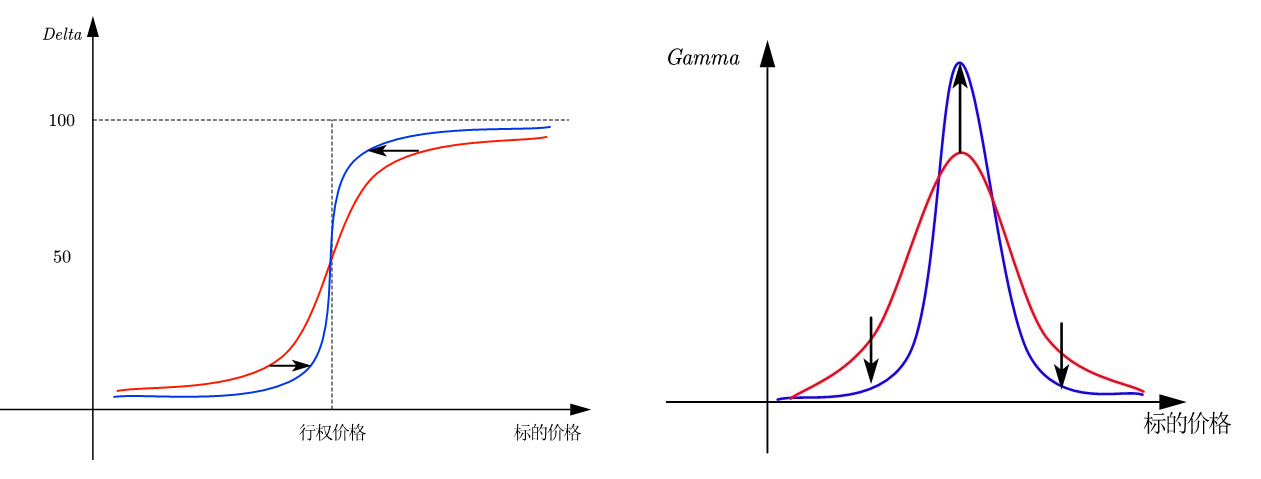
\includegraphics[width=0.8\textwidth]{fig/fig1.png}
    \caption{Fig1}
\end{figure}

\end{itemize}

\noindent \textbf{Theta} \par 
\begin{itemize}
\item Theta通常是负的.
\item Theta值在平值时绝对值最大, 深度实值或深度虚值时绝对值较小.
\item 期权价值与|Theta|在临近到期时的变化见Fig2.
\begin{figure}[H]
    \centering
    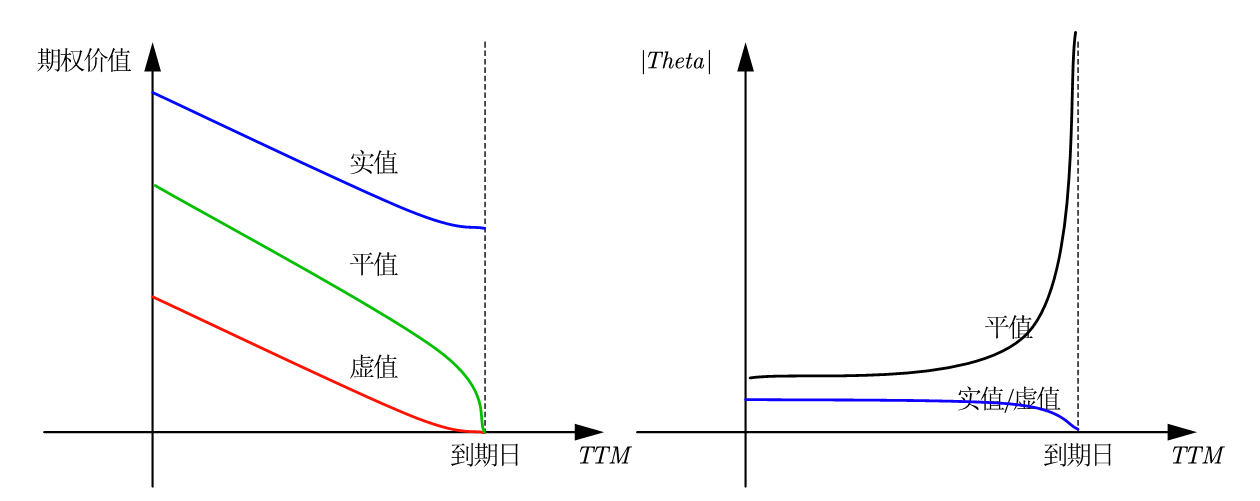
\includegraphics[width=0.7\textwidth]{fig/fig2.png}
    \caption{Fig2}
\end{figure}
\item 平值期权的Theta与波动率成比例变化.
\end{itemize}


\noindent \textbf{Vega} \par 
\begin{itemize}
\item Vega在平值时最大, 深度实值或深度虚值时较小.
\item 期权价值与Vega在不同波动率下的情况见Fig3.
\begin{figure}[H]
    \centering
    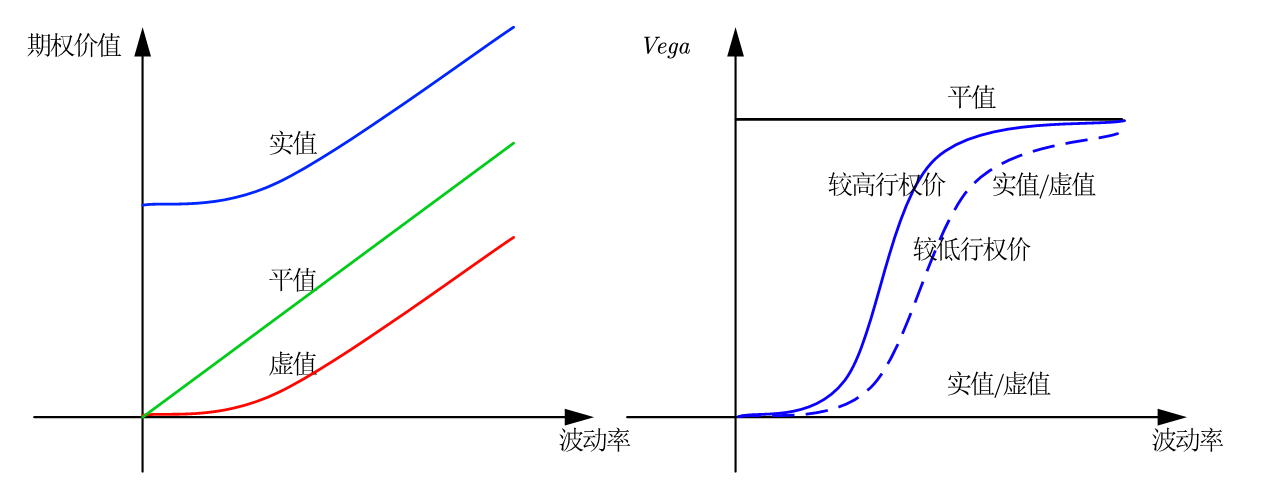
\includegraphics[width=0.7\textwidth]{fig/fig3.png}
    \caption{Fig3}
\end{figure}
\item Vega值随到期日临近的变化见Fig4.
\begin{figure}[H]
    \centering
    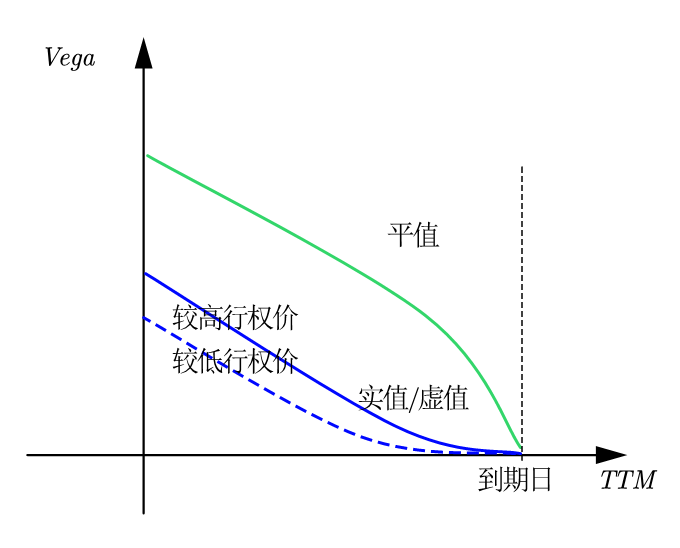
\includegraphics[width=0.4\textwidth]{fig/fig4.png}
    \caption{Fig4}
\end{figure}

\end{itemize}


\subsection{Structure}


\noindent \textbf{对称策略} \par 

以下默认期权多头. 价指Strike Price.

跨式期权 Straddle: Long 同价的Call+Put.
\textbackslash / 形.
Neutral Delta, Long Gamma, Long Vega, Short Theta.

宽跨式期权 Strangle: Long 高价Call + 低价Put.
\textbackslash \_ / 形.
Neutral Delta, Long Gamma, Long Vega, Short Theta.

蝶式期权 Fly: Long 低价Call + 高价Call, Short 2 中间价Call.
\_ / \textbackslash \_ 形.
Neutral Delta, Short Gamma, Short Vega, Long Theta.

鹰式期权 Iron Condor: Long 低价Call + 高价Call, Short 中低价Call+中高价Call.
\_ / - \textbackslash \_ 形.
Neutral Delta, Short Gamma, Short Vega, Long Theta.

\noindent \textbf{时间价差} \par 
时间价差多头: 买入长期期权, 卖出短期期权.(因为长期期权通常更贵)
使用平值期权1:1构成Delta中性.

时间价差多头是Short Gamma的, 因为若标的价格不变, 随时间流逝, 短期期权价值减少是多于长期期权的.

时间价差多头是Long Vega的, 因为波动率变化(上升)对长期期权有更大影响(增加更多时间价值).

\begin{figure}[H]
    \centering
    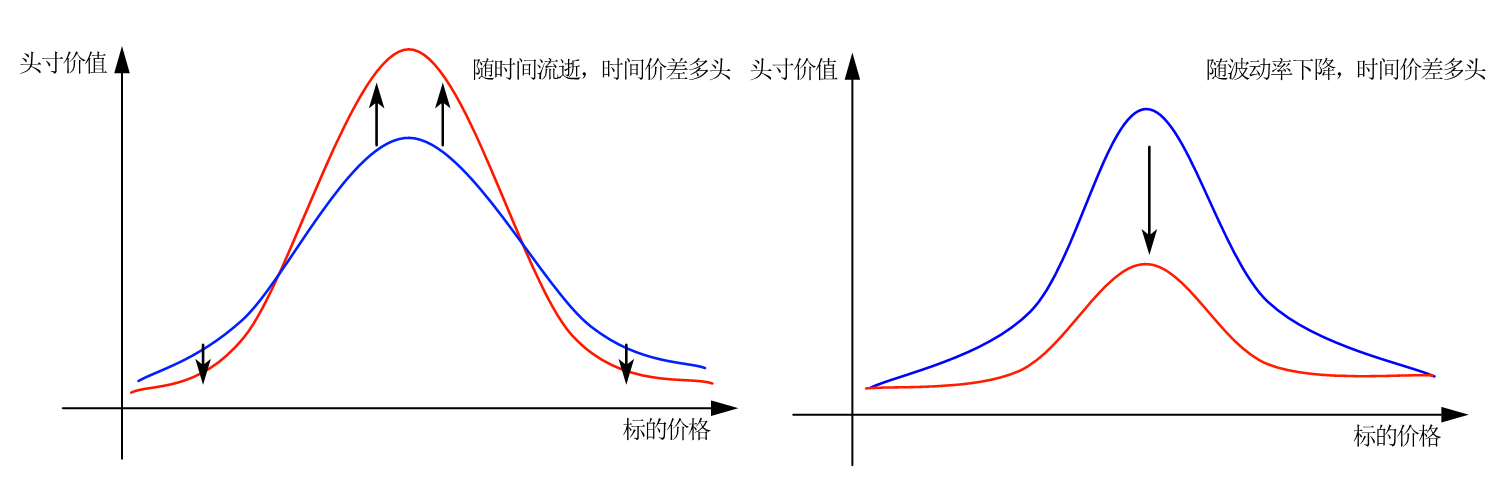
\includegraphics[width=0.7\textwidth]{fig/fig5.png}
    \caption{Fig5}
\end{figure}

策略选择: 如果隐含波动率低, 要 Long Vega.
当隐含波动率很低但被认为会升高时, 时间价差多头可能获利.

\noindent \textbf{垂直价差} \par 
买入与卖出相同类型、同时到期、行权价格不同的期权.
牛市价差 Call Spread: 买低, 卖高. (Call:牛市看涨, Put:牛市看跌).
熊市价差 Put Spread: 卖低, 买高. (Call:熊市看涨, Put:熊市看跌).

买低卖高, 无论是Call还是Put都具有牛市特征, 即具有正的Delta值. 
两个行权价之间差距越大, 牛市特征越明显(价差的Delta越大).

Call Spread Collar: CS + underwrite.
Put Spread Collar: PS + overwrite.

Risk reversal: Buy downside put, partially funded by selling an upside call, or vice versa.

\begin{figure}[H]
    \centering
    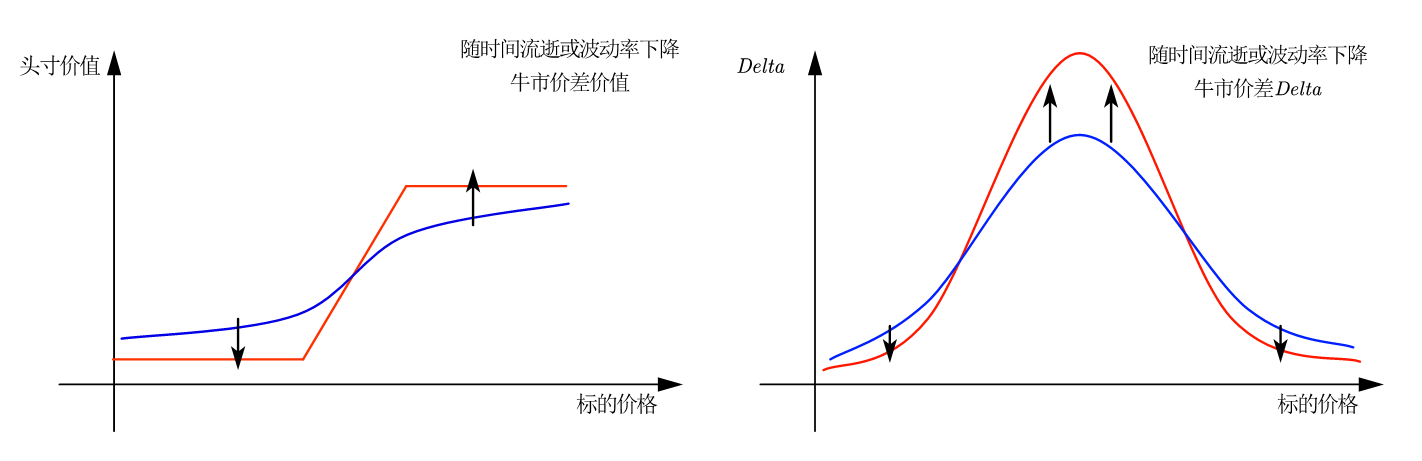
\includegraphics[width=0.7\textwidth]{fig/fig6.png}
    \caption{Fig5}
\end{figure}


\subsection{其他}
\noindent \textbf{美式期权} \par
看涨期权价值=内在+波动率+利率-股利. 因此美式看涨若提前行权, 只可能在股利支付前一天.
看跌期权价值=内在+波动率-利率+股利. 因此美式看跌若提前行权, 要距离除息日足够远, 且波动率价值较小.
无论看涨看跌, 越是实值, 美式与欧式价格差越大; 波动率越小, 美式与欧式价格差越大.


\noindent \textbf{结构化} \par
Down and out + Down and in = Vanilla Call.

Knock-in: Structure is activated after being knocked in (before that coupon is protected).

Knock-out: Immediate termination of structure.

雪球是什么: FCN-KI autocallable (fixed coupon note kick-in variant)


\section{Linear Algebra}

\subsection{矩阵性质}

\begin{itemize}

\item $|\boldsymbol{A B}|=|\boldsymbol{A}||\boldsymbol{B}|$, $|k\boldsymbol{A}|=k^n|\boldsymbol{A}|$

\item $(k \boldsymbol{A})^{-1}=k^{-1} \boldsymbol{A}^{-1}$, $|\boldsymbol{A}^{-1}|=|\boldsymbol{A}|^{-1}$

\item $\operatorname{tr}(\boldsymbol{A} \boldsymbol{B})=
\operatorname{tr}(\boldsymbol{B} \boldsymbol{A})$,
$\operatorname{tr}\left(\boldsymbol{A} \boldsymbol{A}^{\prime}\right)
\geq \operatorname{tr}\left(\boldsymbol{A}^2 \right)$.

\item 若 $\boldsymbol{A}$ 是 $n$ 阶实矩阵, 
则 $\operatorname{tr}\left(\boldsymbol{A} \boldsymbol{A}^{\prime}\right) \geq 0$,
等号成立$\Leftrightarrow\boldsymbol{A}=\boldsymbol{O}$\par

\item $r(\boldsymbol{A} \boldsymbol{B}) \leq \min \{r(\boldsymbol{A}), r(\boldsymbol{B})\}$;\par

\item $r(\boldsymbol{A}+\boldsymbol{B}) \leq r(\boldsymbol{A})+r(\boldsymbol{B}), 
r(\boldsymbol{A}-\boldsymbol{B}) \leq r(\boldsymbol{A})+r(\boldsymbol{B})$;\par

\item Sylvester不等式.
设$\boldsymbol{A}$是$m\times n$矩阵,$\boldsymbol{B}$是$n\times t$矩阵,则
$r(\boldsymbol{A} \boldsymbol{B}) \geq r(\boldsymbol{A})+r(\boldsymbol{B})-n$.

\item 设$\boldsymbol{A}$是$m\times n$阶实矩阵,则
$r\left(\boldsymbol{A}^{\prime} \boldsymbol{A}\right)=
r\left(\boldsymbol{A} \boldsymbol{A}^{\prime}\right)=r(\boldsymbol{A})$

\item 设$\boldsymbol{A}$是$m\times n$矩阵,则:\par
$(1)$若$r(\boldsymbol{A})=n$,即$\boldsymbol{A}$列满秩,则必存在秩等于$n$的
$n\times m$矩阵$\boldsymbol{B}$使$\boldsymbol{B}\boldsymbol{A}=\boldsymbol{I}_{n}$;\par
$(2)$若$r(\boldsymbol{A})=m$,即$\boldsymbol{A}$行满秩,则必存在秩等于$m$的
$n\times m$矩阵$\boldsymbol{C}$使$\boldsymbol{AC}=\boldsymbol{I}_{m}$.

\item 满秩分解.
设$\boldsymbol{A}$是秩为r的$m\times n$矩阵,则有满秩分解$\boldsymbol{A}=\boldsymbol{B}\boldsymbol{C}$,
其中$\boldsymbol{B}$是秩为r的$m\times r$矩阵,$\boldsymbol{C}$是秩为r的$r\times n$矩阵.

\item 设$A$是$n$阶幂等矩阵,则存在n阶非异阵$\boldsymbol{P}$,使得$\boldsymbol{P}^{-1} \boldsymbol{A P}=\left(\begin{array}{ll}\boldsymbol{I}_{r} & \boldsymbol{O} \\ \boldsymbol{O} & \boldsymbol{O}\end{array}\right)$,
其中$r=\mathrm{r}(\boldsymbol{A})$ 

\end{itemize}


\subsection{特征值}

\begin{itemize}

\item 任一复方阵必相似于一上三角阵,且主对角线上元素为特征值.

\item 若$A$特征值为$\lambda_1,\cdots,\lambda_n$,则$f(A)$的特征值为$f(\lambda_1),\cdots,f(\lambda_n)$.
若$A$适合多项式$g(x)$,则$A$的任意特征值适合$g(x)$.

\item 特征值降阶公式.
设A是$m \times n$矩阵,B是$n \times m$矩阵,且$m \geq n$.则
$\left|\lambda I_{m}-A B\right|=\lambda^{m-n}\left|\lambda I_{n}-B A\right|$

\item 可对角化判定方法\par 
充分条件: 有 $n$ 个不同的特征值, 相似于实对称阵\par 
充要条件: 有n个线性无关的特征向量, 极小多项式无重根, 初等因子都是一次多项式或Jordan块都是一阶矩阵

\item Jordan标准型求法\par 
$\lambda I-A$相抵于$\operatorname{diag}\{1,\dots,1,d_1(\lambda),\dots,d_k(\lambda)\}$, 对角元$d_i | d_{i+1}$.
$d_1,\dots,d_k$的准素因子全体(初等因子)对应Jordan块拼起来即为Jordan标准型.

\item $J=J_r(\lambda )$为Jordan块.则$f(J)$主对角线上元素均为$f(\lambda )$,上次对角线上元素均为$f'(\lambda)$.
距离主对角线j位的对角平行线上的元素均为$\frac{1}{j!}f^{(j)}(\lambda)$.
对$\lambda\neq 0$,则$J_r(\lambda)^m$的Jordan标准型为$J_r(\lambda^m)$

\item $A^k$求法: 先求出Jordan标准型$J$, 根据$AP=PJ$解方程得$P$, 求$J^k$再乘过渡矩阵即可.

\end{itemize}


\subsection{二次型}

\begin{itemize}
\item 设$A$为$n$阶实对称阵,则以下结论等价:\par
$(1)$$A$正定\quad $(2)$$A$合同于$I_n$\quad $(3)$存在非异实矩阵$C,A=C'C$\quad $(4)$$A$的主子式都大于$0$\par 
$(5)$$A$的顺序主子式都大于$0$\quad $(6)$$A$的特征值都大于$0$.

\item $\boldsymbol{A}=\left(a_{i j}\right)$是$n$阶半正定实对称矩阵,则$|\boldsymbol{A}| \leq a_{11} a_{22} \cdots a_{n n}$,
等号成立当且仅当 $\boldsymbol{A}$ 是对角矩阵或某个$a_{ii}=0$.

\item 设$\boldsymbol{A}$为n阶实对称矩阵,则$\boldsymbol{A}$半正定或半负定$\Leftrightarrow$
对任意$\boldsymbol{\alpha}$满足$\boldsymbol{\alpha}^{\prime} \boldsymbol{A} \boldsymbol{\alpha}=0$,
均有$\boldsymbol{A} \boldsymbol{\alpha}=\mathbf{0}$.

\item 若实矩阵$A$满足$A^{\prime}=A^{-1}$,则称$A$为正交阵. A为正交阵/酉阵的充要条件为A的n个行向量构成一组标准正交基.

\item 实对称阵与Hermite阵特征值全为实数,反对称阵特征值全为0或纯虚数.

\item 实对称阵与Hermite阵合同于$\operatorname{diag}\{I_p,-I_q,0\}$.
实对称阵(Hermite阵)正交相似(酉相似)于实对角阵.

\item 复正规阵酉相似于复对角阵,对角元模长都为1.实反对称阵酉相似于复对角阵.

\item Gram-Schmidt正交化方法.
$\{u_1,\dots,u_m\}$为一组线性无关的向量,
令$$v_{k+1}=u_{k+1}-\sum _{i=1}^k\frac{(u_{k+1},v_i)}{\Vert v_i\Vert^2}v_i$$
则$\{v_1,\dots,v_m\}$为一组正交向量.

\end{itemize}

\subsection{一些分解}

\begin{itemize}

\item QR分解\par 
设$A$为n阶实/复矩阵,则$A=QR$,其中$Q$为正交/酉阵,$R$为主对角元均$\geq 0$的上三角阵.若$A$非异,则分解唯一.

\item Jordan-Chevalley分解\par 
设A为n阶复方阵,则有分解$A=B+C$,满足:\par 
$(1)$B可对角化\qquad $(2)$C为幂零阵\qquad $(3)$$BC=CB$\qquad $(4)$B,C可表示为A的多项式\par 
并且满足前三条的分解唯一.

\item Cholesky分解\par 
设A为n阶实对称阵/Hermite阵,若A正定,则存在对角元均为正实数的下三角$(\text{或上三角})$实矩阵L使得$A=LL^{\prime}$/$A=L\overline{L^{\prime}}$,
并且分解唯一.若A为半正定阵,则对角元均为非负数,且分解不一定唯一.

\item 极分解\par 
$\varphi \in \mathcal{L}(V)$,则$\varphi = \omega\psi$.其中$\omega$保积,$\psi$半正定自伴随.若$\varphi $可逆,则分解唯一. \par 
$A\in M_n(R)$,则$A=OS$,其中$O$为正交阵,$S$为半正定实对称阵.\par 
$A\in M_n(C)$,则$A=UH$,其中$U$为酉阵,$H$为半正定Hermite阵.

\item 奇异值分解\par 
$A\in M_{m\times n}(R)$,则$A=P \operatorname{diag}\{S,0\}Q^{\prime}$.
其中$P,Q$为$m,n$阶正交阵,$S=\operatorname{diag}\{\sigma_1,\cdots ,\sigma_r\}$,
$\sigma_1\geq \cdots \geq \sigma_r>0$为$A$的所有奇异值,即$\sigma_1^2,\cdots,\sigma_r^2$为$A^{\prime}A$的非零特征值全体.

\end{itemize}


\subsection{计算}

$A$是实对称阵, 求非异矩阵$C$使得$C'AC$是对角阵: 
作$n\times 2n$矩阵$(A, I_n)$, 实施初等行变换, 并对左侧矩阵实施对应初等列变换,
将左侧化为对角阵. 此时右侧矩阵的即为$C'$.


$A$是实对称阵, 求正交矩阵$P$使得$P'AP$是对角阵: 
求特征值, 对每个特征值$\lambda$, 求解$(\lambda I-A)x=0$得到基础解系.
若基础解系有多个向量, 进行正交化.
所有列向量单位化后拼接得到$P$.

\section{Calculus}

\subsection{一元微积分}
Please see 数分2 notes attached.


\subsection{多元微分}

Hessian matrix: $f$为$\mathbb{R}^n\to\mathbb{R}$函数,
$H(f)=\left(\frac{\partial^2 f}{\partial x_i \partial x_j}\right)_{n\times n}$

Jacobi matrix: $f$为$\mathbb{R}^n\to \mathbb{R}^m$向量值函数,
$J(f)=\left(\frac{\partial f_i}{\partial x_j}\right)_{m\times n}$

Prop. $H(f(x))=J(\nabla f(x))^T$.

Hessian矩阵正定的极值点是极小值点, 负定是极大值点.

隐函数存在定理:
对多元函数$F(x_1,\dots,x_n,y)=0$, 在周围闭矩形连续且有连续偏导, $F_y\neq 0$, 有$\frac{\partial y}{\partial x_i}=-\frac{F_{x_i}}{F_y}$.
多元向量值函数$F(x_0,y_0,u_0,v_0)=0, G(x_0,y_0,u_0,v_0)=0$, Jacobi行列式$\frac{\partial(F,G)}{\partial(u,v)}\neq 0$,
则有$\begin{pmatrix} u_x & u_y \\ v_x  & v_y \end{pmatrix} = -\frac{\partial(F,G)}{\partial(u,v)} ^{-1}\frac{\partial(F,G)}{\partial(x,y)}$.


\noindent \textbf{几何应用}

\noindent 1.曲线$\Gamma: x=x(t),y=y(t),z=z(t)$,
    在$P_0(x_0,y_0,z_0)$处切向量$\vec{\tau}=(x',y',z')\mid _{P_0}$,
    法平面为$x'(x-x_0)+y'(y-y_0)+z'(z-z_0)= 0$.\par 
~\\
\noindent 2.曲线$\Gamma: \left\{\begin{array}{l}
    F(x, y, z)=0 \\ G(x, y, z)=0 \end{array}\right.$,
    在$P_0(x_0,y_0,z_0)$处切向量$\vec{\tau}=(\frac{\partial (F,G)}{\partial (y,z)},
    \frac{\partial (F,G)}{\partial (z,x)}, \frac{\partial (F,G)}{\partial (x,y)})
    \mid _{P_0}$,法平面为$\operatorname{grad}F(P_0),\operatorname{grad}G(P_0)$张成的平面.\par 
~\\
\noindent 3.曲面$F(x,y,z)=0$在$P_0(x_0,y_0,z_0)$处法向量$\vec{n}=(F_x,F_y,F_z)\mid _{P_0}$,
    切平面为$\frac{x-x_0}{F_x(P_0)}=\frac{y-y_0}{F_y(P_0)}=\frac{z-z_0}{F_z(P_0)}$.\par 
~\\
\noindent 4.曲面$x=x(u,v),y=y(u,v),z=z(u,v)$,法向量$\vec{n}=(
    \frac{\partial (y,z)}{\partial (u,v)},\frac{\partial (z,x)}{\partial (u,v)},\frac{\partial (x,y)}{\partial (u,v)})$.


\subsection{重积分}

重积分变量代换:
映射$T:
\left\{\begin{matrix}
x=x(u,v)\\y=y(u,v)
\end{matrix}\right.,D\to T(D)$
有连续偏导且$\frac{\partial(x,y)}{\partial(u,v)}\neq 0$.
$f(x,y)$在$T(D)$连续, 则
$\iint_{T(D)}f(x,y)\mathrm{d}x\mathrm{d}y=\iint_{D} f(x(u,v), y(u,v))
\left|\frac{\partial(x,y)}{\partial(u,v)}\right| \mathrm{d}u\mathrm{d}v$


\noindent 常用变量代换:\par 
极坐标变换$x=r\cos\theta,y=r\sin\theta$下$\mathrm{d}x\mathrm{d}y=r\mathrm{d}r\mathrm{d}\theta$.\par 
柱坐标变换$x=r\cos\theta,y=r\sin\theta,z=z$下$\mathrm{d}x\mathrm{d}y\mathrm{d}z=r\mathrm{d}r\mathrm{d}\theta\mathrm{d}z$.\par 
球坐标变换$x=r\sin\varphi\cos\theta,y=r\sin\varphi\sin\theta,z=r\cos\varphi,
r\in[0,+\infty),\varphi\in[0,\pi],\theta\in[0,2\pi]$下$\mathrm{d}x\mathrm{d}y\mathrm{d}z
=r^2\sin\varphi \mathrm{d}r\mathrm{d}\varphi \mathrm{d}\theta$.\par 
广义球坐标变换$x=ar\sin\varphi\cos\theta,y=br\sin\varphi\sin\theta,z=cr\cos\varphi$下$\mathrm{d}x\mathrm{d}y\mathrm{d}z
=abcr^2\sin\varphi \mathrm{d}r\mathrm{d}\varphi \mathrm{d}\theta$.\par 
n重球坐标变换$x_{1}=r \cos \varphi_{1}, x_{2}=r \sin \varphi_{1} \cos \varphi_{2}, \cdots,
x_{n-1}=r \sin \varphi_{1}\cdots \sin \varphi_{n-2} \cos \varphi_{n-1},
x_{n}=r \sin \varphi_{1}\cdots\sin \varphi_{n-1},
0\leq \varphi_1,\cdots,\varphi_{n-2}\leq \pi,0\leq \varphi_{n-1}\leq 2\pi$下$
\frac{\partial\left(x_{1}, x_{2}, \cdots, x_{n}\right)}{\partial\left(r, \varphi_{1}, \cdots, \varphi_{n-1}\right)}=
r^{n-1} \sin ^{n-2} \varphi_{1}$
$\sin ^{n-3} \varphi_{2} \cdots \sin \varphi_{n-2} $.

\subsection{曲线与曲面积分}
Please see 数分3 notes attached.

\section{常微}

\noindent 1. 分离变量 \par 
(1)齐次方程$\frac{dx}{dt}=f(\frac{x}{t})$. 令$\frac{x}{t}=u$,则$\frac{du}{dt}t=f(u)-u$.\par 
(2)$\frac{dx}{dt}=f(at+bx+c)$. 令$y=at+bx+c$,则$\frac{dy}{dt}=a+bf(y)$.\par 
~\\

\noindent 2. 非齐次线性方程 $\frac{dx}{dt}=P(t)x+Q(t)$\par 
常数变易,两边乘$e^{-\int P(t)dt}$. 常数变易公式$x=e^{\int P(t)dt}(\int e^{-\int P(t)dt}Q(t)dt+C)$.
~\\


\noindent 3. 全微分方程 $M(t,x)dt+N(t,x)dx=0$ \par 
(1) $\frac{\partial M(t,x)}{\partial x}=\frac{\partial N(t,x)}{\partial t}$, 则存在$u(t,x)$使得$du(t,x)=M(t,x)dt+N(t,x)dx$\par 
设$u(t,x)=\int M(t,x)dt+\varphi(x)$,由$N(t,x)=\frac{\partial }{\partial x}\int M(t,x)dt+\varphi'(x)$可求出$\varphi(x)$. \par 
(2) $\frac{\partial M(t,x)}{\partial x} \neq \frac{\partial N(t,x)}{\partial t}$, 
要找积分因子$\mu$使得$\frac{\partial \mu M}{\partial x}=\frac{\partial \mu N}{\partial t}$ \par 
可寻找特殊形式的$\mu(t,x) $,如取$\mu (x),\mu (t),\mu (xt),\dots $,代入$\frac{\partial \mu M}{\partial x}=\frac{\partial \mu N}{\partial t}$ 求解.
~\\


\noindent 4. 导数未解出的一阶方程 \par 
$x=f(t,\frac{dx}{dt})$或$t=f(x,\frac{dx}{dt})$,
引入$p=\frac{dx}{dt}$求解.
~\\


\noindent 5. 高阶方程的降阶 \par 
(1)不含$x$,$F\left(t, x^{(k)}, \cdots, x^{(n)}\right)=0$.
令$x^{(k)}=y$,则化为$F\left(t, y, \cdots, y^{(n-k)}\right)=0 $.\par 
(2)不含$t$,$F\left(x, \frac{d x}{d t}, \cdots, \frac{d^{n} x}{d t^{n}}\right)=0$.
引入$y=\frac{dx}{dt}$,以$x$为新自变量.则$x^{(k)}$可用$y,\frac{dy}{dx},\cdots,\frac{d^{k-1}y}{dx^{k-1}}$表示.\par 
~\\

\noindent 6. 齐次常系数线性方程
$x^{(n)}+a_1x^{(n-1)}+\cdots +a_{n-1}x^{(1)}+a_nx=0$ \par 
特征方程$\lambda ^{n}+a_1\lambda^{n-1}+\cdots +a_{n-1}\lambda+a_n=0$.
$\lambda_1,\dots ,\lambda_s$为不同实根,重数$n_1,\dots ,n_s$,
$\alpha_1 \pm i\beta_1,\dots ,\alpha_p \pm i\beta_p$为共轭虚根,重数为$m_1,\dots ,m_p$.
则实值通解$$x(t)=\sum_{i=1}^s P_i(t)e^{\lambda_i t} + \sum_{i=1}^p e^{\alpha_i t}(W_i(t)\cos \beta_i t +V_i(t) \sin\beta_i t)$$ \par 
其中$P_i(t)$为$n_i-1$次实系数多项式,$W_i(t),V_i(t)$为$m_i-1$次实系数多项式.
~\\

\noindent 7. 非齐次常系数线性方程
$x^{(n)}+a_1x^{(n-1)}+\cdots +a_{n-1}x^{(1)}+a_nx=f(t)$ \par 
解为$x(t)=x_1(t)+x^*(t)$,其中$x_1(t)$为$x^{(n)}+a_1x^{(n-1)}+\cdots +a_{n-1}x^{(1)}+a_nx=0$的通解,
$x^*(t)$为$x^{(n)}+a_1x^{(n-1)}+\cdots +a_{n-1}x^{(1)}+a_nx=f(t)$的特解. \par 
$x^*(t)=\int _0^t K(t-s)f(s)ds$,其中$K(t)$为$x^{(n)}+a_1x^{(n-1)}+\cdots +a_{n-1}x^{(1)}+a_nx=0$
在初值条件$K(0)=K'(0)=\cdots =K^{(n-1)}(0)=0, K^{(n)}(0)=1$下的解.
~\\

\noindent 8. Euler方程
$t^nx^{(n)}+a_1t^{n-1}x^{(n-1)}+\cdots +a_{n-1}tx^{(1)}+a_nx=0$ \par 
引入$s=\ln |t|$,记$D_s=\frac{d}{ds}$,则$t^n x^{(n)}=D_s(D_s-1)\cdots (D_s-n+1)x$.
~\\

\noindent 9. 齐次常系数线性微分方程组$\frac{d\vec{x}}{dt}=A\vec{x} $ \par 

若$A$可对角化,则$\vec{x}(t)=\sum _{i=1}^n c_i e^{\lambda_i t}\vec{p_i}$,$\vec{p_i}$为$\lambda_i$的特征向量. \par 
若A有复数特征值$\lambda=\alpha+i\beta$和$\bar{\lambda}=\alpha-i\beta$,
则方程组实值解形如$\vec{x}=e^{\alpha t}\{\vec{p}(t) \cos \beta t+\vec{q}(t) \sin \beta t\}$,
其中$\vec{p}(t)$和$\vec{q}(t)$是$t$的次数小于$\lambda$重数的实向量多项式,其向量系数由微分方程组确定. \par 

对一般矩阵$A$,Jordan标准型为$J$,$P^{-1}AP=J$,则$\vec{x}(t)=Pe^{Jt}\vec{c}$,
其中对$\lambda_i$的Jordan块$J_i$,$e^{J_it}$第一行为$e^{\lambda_it},te^{\lambda_it},\dots ,\frac{t^{n_i-1}}{(n-1)!}e^{\lambda_it}$.
记$\vec{p}_i$为$P$的第$i$个列向量,则有 \par 
$\vec{x}(t)= \sum_{i=1}^{s}\left\{c_{i_1}e^{\lambda_it} \vec{p}_{i_1}+c_{i_2}\left[te^{\lambda_it} \vec{p}_{i_1}+e^{\lambda_it}\vec{p_{i_2}}\right]
+\cdots+c_{i_{n_{i}}}\left[\frac{t^{n_{i}-1}}{\left(n_{i}-1\right)!} e^{\lambda i t} \vec{p_{i_1}}+\cdots+e^{\lambda_it} \vec{p}_{i_{n_{i}}}\right]\right\}$.\par 
$\forall \operatorname{Re}\{\lambda_i\}<0 \Leftrightarrow \|\vec{x}(t)\| \leq M$.
~\\

\noindent 10. 非齐次常系数线性微分方程组$\frac{d\vec{x}}{dt}=A\vec{x} +\vec{f}(t)$ \par 
方程的解$\vec{x}(t)=Pe^{Jt}\vec{c(t)}=Pe^{Jt}\vec{c}+\int_{0}^te^{A(t-s)}\vec{f}(s)ds$ \par 
对初值问题$\vec{x}(t_0)=\vec{x_0}$,有$\vec{x}(t)=e^{A(t-t_0)}\vec{x_0}+\int_{t_0}^te^{A(t-s)}\vec{f}(s)ds$.
~\\


\section{Others}

\subsection{矩阵范数}

Frobenius范数$\| A\|=\sqrt{\sum_{i,j}a_{ij}^2}$

由向量范数$\| \vec{x}\| _p=(\sum _i |x_i|^p)^{1/p}$诱导的矩阵范数$\| A\|_p=\operatorname{sup}
_{\vec{x}\neq \vec{0}} \frac{\| A\vec{x} \|_p}{\| \vec{x} \|_p}$.


$\|A\|_{1}=\max _{1 \leqslant j \leqslant n}\left\{\sum_{i=1}^{n}\left|a_{i j}\right|\right\},
\|A\|_{2}=\sqrt{\lambda_{\max} \left(A^T A\right)},
\|A\|_{\infty}=\max _{1 \leqslant i \leqslant n}\left\{\sum_{j=1}^{n}\left|a_{i j}\right|\right\}$. \par 

由向量范数诱导的矩阵范数有性质
(1)$\|A \vec{x}\| \leqslant\|A\| \cdot\|\vec{x}\|$ \quad 
(2)$\|A\|=\sup _{\|\vec{x}\|=1}\|A \vec{x}\|$ \quad 
(3)$\|A B\| \leqslant\|A\| \cdot\|B\|$ \quad 
(4)$\left\|\int_{\alpha}^{\beta} A(s) d s\right\| \leqslant\left|\int_{\alpha}^{\beta}\|A(s)\| d s\right|$
~\\

矩阵指数函数: $(e^{At})^{-1}=e^{-At}$, $e^{A(t+s)}=e^{At}\cdot e^{As}$.


\subsection{矩阵求导}
关于$t$求导与积分:对矩阵每个元素求导与积分.

$\frac{d}{dt}[A(t)B(t)]=A'(t)B(t)+A(t)B'(t)$.

将矩阵$X_{m\times n}$按列堆栈向量化, $vec(X)=[x_{11},\dots,x_{m1},\dots,\dots,x_{mn}]^T$.
将矩阵函数$F:m\times n\to p\times q$向量化, $vec(F(X))=[f_{11}(X),\dots,f_{p1}(X),\dots,\dots,f_{pq}(X)]^T$.

$D_X F(X)=\frac{\partial vec_{pq\times 1}(F(X))}{\partial vec_{mn\times 1}^T X} \in \mathbb{R}^{pq\times mn}$.


向量变元标量函数:
$\frac{\partial a^Tx}{\partial x}=a$,
$\frac{\partial x^TAx}{\partial x}=Ax+A^Tx$,
$\frac{\partial a^T xx^T b}{\partial x}=ab^Tx+ba^Tx$.

矩阵变元标量函数
$\frac{\partial a^T X b}{\partial X}=ab^T$,
$\frac{\partial a^T XX^T b}{\partial X}=ab^TX+ba^TX$.



\end{document}
